\section{Results and Discussion}
\label{Sec:Res}
In this section, the proposed method using dataset a, b, c are compared to the recent non-deep-learning algorithms, such as Minh-CNN\cite{IEEEexample:mnih2013machine}, Satio-multi\cite{IEEEexample:saito2016multiple}, Context\cite{IEEEexample:audebert2017deep}. In addition, our method is compared with some recent deeplearning based approaches, including FCN\cite{IEEEexample:Long_2015_CVPR}, SegNet\cite{IEEEexample:badrinarayanan2017segnet} and etc. Moreover for HF-FCN itself, we expect to investigate the effects of extracted information from different layers on the final prediction. Hence, some variants which combine different up-sampling feature maps from Level 2 are proposed with details shown in Figure 6.\par

\begin{figure}[t]
\begin{center}
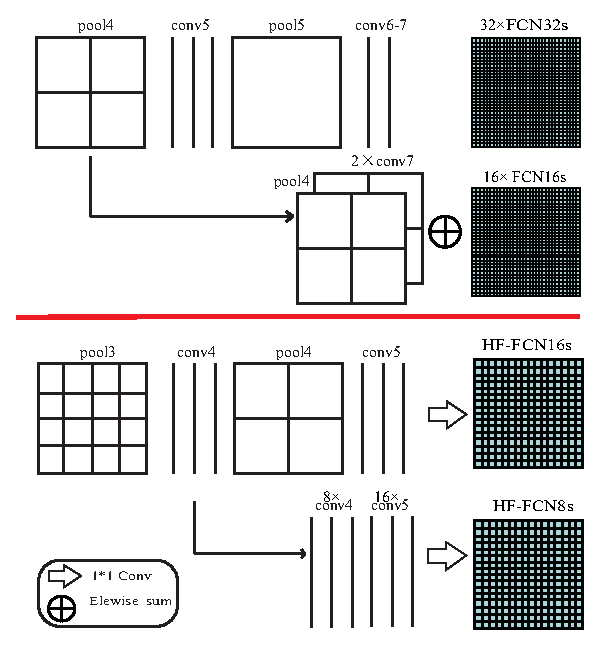
\includegraphics[width=7.8cm]{Figures/vairants.eps}
\caption{HF-FCN variants. The feature maps generated from final group are fused into a coarse result, which is HF-FCN16s. The variant called HF-FCN8s concatenates the feature maps from the last 2 groups with the same fusion operation, and so on.}
\label{6}
\end{center}
\end{figure}

\subsection{Massachusetts dataset}
On the Massachusetts dataset, our method is compared to three state-of-the-art approaches. Table 4 and Figure 7 present the quantitative analysis and precision-recall curves respectively. A standard and relaxed precision and recall are amply to make a comparison. From the reuslt, our method shows obvious superiority in terms of speed and precision. When comparing with Satio\-multi\-MA\&CIS, standard and relaxed recall are 5.5{\%} and 1.3{\%} higher than it, respectively. And, at the same time, the time coat is reduced from 67.84s to 1.07s, the speed is up about 63 times. These significant improvements demonstrate that HF-FCN achieves best performance in effectiveness and efficiency.\par
\setlength{\parindent}{2ex}Meanwhile, extensive comparisons are made between HF-FCN and other mainstream methods in semantic segmentation domain. The visual results are shown in Figure 10. From it, we can see that details and integrity of the building are well preserved by using our method.
\begin{table}
\centering
\caption {Correctness at breakeven of HF-FCN v.s. \cite{IEEEexample:mnih2013machine}\cite{IEEEexample:saito2016multiple}\cite{IEEEexample:alshehhi2017simultaneous} on Massachusetts test set. Cost time is computed in the same computer with a single NVIDIA Titan 12GB GPU}
\begin{tabular}{cccc}
\hline
&Recall ($\rho$ = 3)&Recall ($\rho$ = 0)&Time (s)\\
\hline
Mnih-CNN [9]&0.9271&0.7661&8.70\\
Mnih-CNN+CRF [9]&0.9282&0.7638&26.60\\
Satio-multi-MA [10]&0.9503&0.7873&67.72\\
Satio-multi-MA\&CIS [10]&0.9509&0.7872&67.84\\
Alshehhi-GAP+seg [11]&0.955&{--}&{--} \\
Proposed model (HF-FCN)&0.9643&0.8424&1.07\\ \hline
\end{tabular}
\end{table}

\begin{figure}
\centering
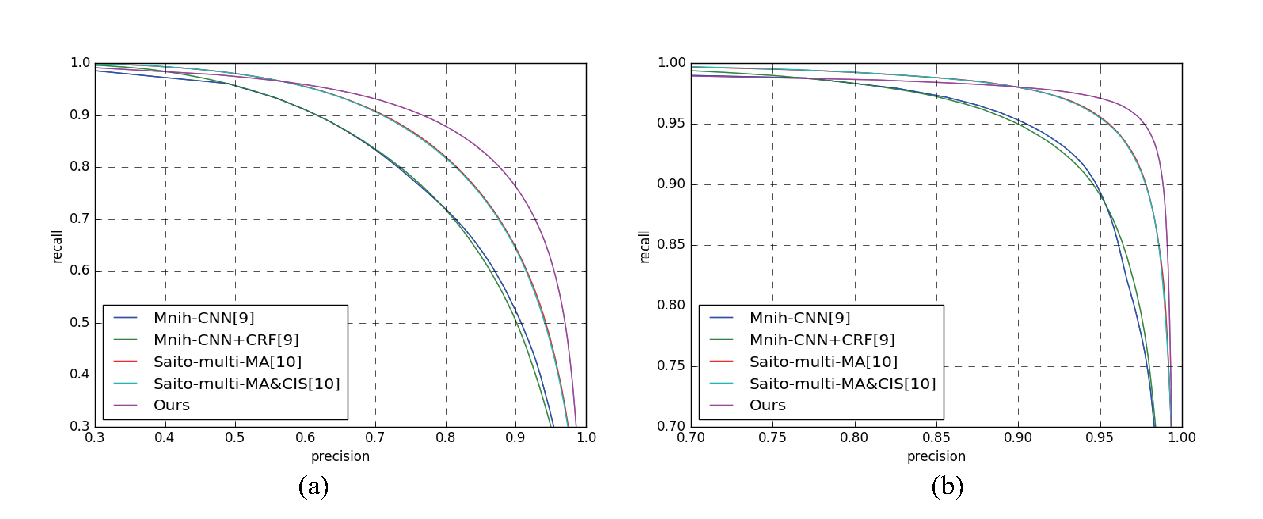
\includegraphics[width=8.7cm]{Figures/HF-FCN_dataset_a.eps}
\caption{The relaxed precision-recall curves from different methods with two slack paramters, (a) $\rho$ = 0; (b) $\rho$ = 3. All curves of our model are located above others.}
\label{7}
\end{figure}
\setlength{\parindent}{2ex}To explore the effects of the feature maps at different scales on the final result, variants of HF-FCN which are counterpart of FCN are designed. Unlike FCN, a fusion operation rather than summing up components in respective locations are leveraged to build our HF-FCN 16s, 8s, 4s. The performance of these variants are shown in Figure 8, Figure 9 and Table \Rmnum{5}. From the disgrams, we get the following conclusions. First, the prediction result obtained from the last layer gets a coarse result, which losts much of location information that mainly encoded in the shallow feature maps. Second, the largest gap presented between HF-FCN16s and HF-FCN8s about 9{\%} in recall rates, it may suggest that the most information supplement to the HF-FCN is got in middle layers. Third, the PR curves of HF-FCN4s and HF-FCN almost coincide. It illustrates the low-level information has little effect on the prediction results. Forth, with the addition of the shallow feature map, the network is more distinct for the segmentation of tiny buildings, which solves the problem of easy adhesion to adjacent buildings. Since, all the Conv layers contained useful hierarchical information that is critical to the final prediction.\par
\begin{table}
\centering
\caption {Performance comparison between HF-FCN variants on Massachusetts test set.}
\begin{tabular}{ccc}
\hline
&Recall ($\rho$ = 3)&Recall ($\rho$ = 0)\\
\hline
HF-FCN16s&0.9330&0.7233\\
HF-FCN8s&0.9643&0.8171\\
HF-FCN4s&0.9632&0.8394\\
HF-FCN&0.9643&0.8394\\
\hline
\end{tabular}
\end{table}

\begin{figure}
\centering
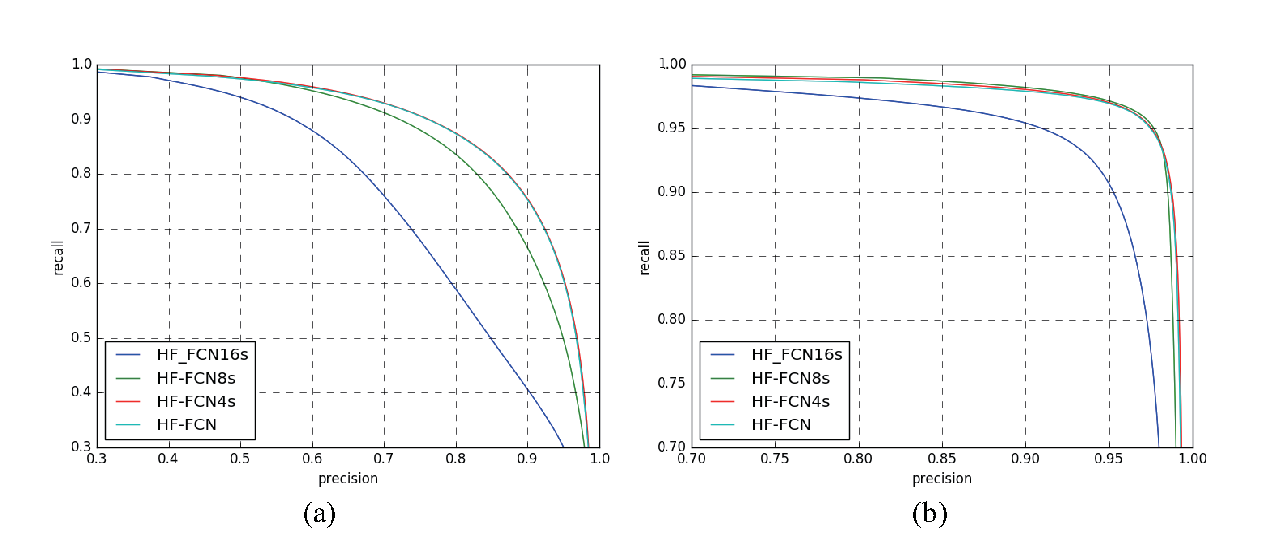
\includegraphics[width=8.7cm]{Figures/HF-FCN-variant-PR.eps}
\caption{The relaxed precision-recall curves from HF-FCN variants with two slack paramters. The biggest gap occurs between HF-FCN16s and HF-FCN8s, which indicates the most additional information coming from middle layers.}
\label{8}
\end{figure}

\begin{figure}
\centering
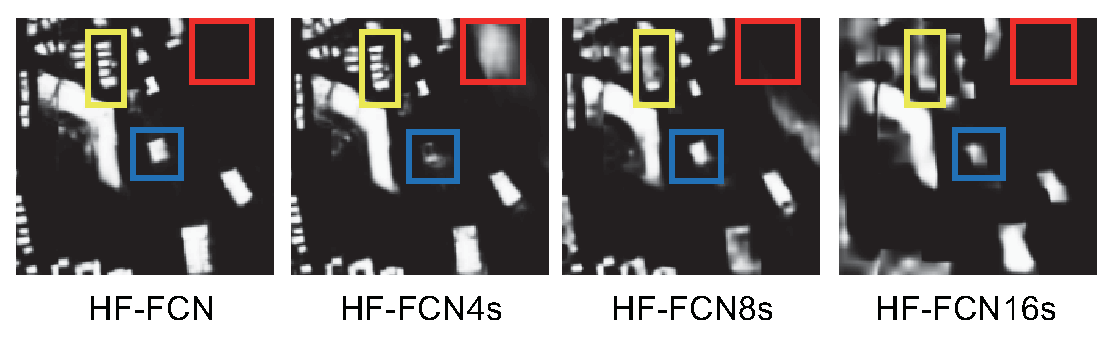
\includegraphics[width=8.7cm]{Figures/HF-FCN_variants_result.eps}
\caption{Prediction results of HF-FCN, HF-FCN4s, HF-FCN8s and HF-FCN16s. The yellow box shows the continuous refinement of the tiny buildings. The red and blue boxes show the mutual promotion and contradiction between different layers.}
\label{9}
\end{figure}

\begin{figure*}
\centering
\includegraphics[width=16.5cm]{Figures/mass_visi_result.eps}
\caption{(a) input images. (b) Results of Mnih-CNN+CRF. (c) Results of Satio\-multi\-MA\&CIS. (d) Results of FCN4s . (e) Results of SegNet. (f) Our results. TP are shown in green, FP are shown in blue and FN are in red.}
\label{10}
\end{figure*}

\subsection{Vaihingen dataset}
On Vaihingen dataset, three experiments are undertaken to explore the effects of different inputs, diverse variants and various methods. We utilize  three kinds of combinations of image channels as inputs. The inputs of the 3 channels are IR, R, G and adding the nDSM as the forth channel. Based on it, DSM is added and made up 5-channel input. We use three standards to make a more comprehensive evaluation. The evaluation results are shown in Table \Rmnum{6}, which illustrates that 3-channel input performed better than the other. Corresponding visual results are shown in Figure 13.\par
\begin{table*}[htbp]
\caption {Performance comparison of the results of different inputs on Vaihigen data set}
\centering
\begin{tabular}{p{1.1cm}<{\centering}|p{1.1cm}<{\centering}|p{1.1cm}<{\centering}|p{1.1cm}<{\centering}|p{1.1cm}<{\centering}|p{1.1cm}<{\centering}|p{1.1cm}<{\centering}|p{1.1cm}<{\centering}|p{1.1cm}<{\centering}|p{1.1cm}<{\centering}|p{1.1cm}<{\centering}}
\hline
&\multirow{2}{*}{Img}&\multicolumn{3}{c}{3\_in: IR, R, G} &\multicolumn{3}{|c|}{4\_in: IR, R, G, nDSM}&\multicolumn{3}{c}{5\_in: IR, R, G, DSM, nDSM}\\
\cline{3-11}
&& Pre &Rec & F1 &Pre &Rec &F1&Pre &Rec &F1\\
\hline
\multirow{3}{*}{Val}&11&0.911&0.906&0.909&0.936&0.900&0.917&0.890&0.900&0.900\\
&28&0.94&0.875&0.906&0.96&0.792&0.868&0.952&0.823&0.883\\
&34&0.965&0.899&0.930&0.987&0.902&0.942&0.972&0.918&0.944\\
&Ave&0.939&0.894&$\bm{0.915}$&0.961&0.865&0.909&0.939&0.880&0.907\\
\hline
\multirow{2}{*}{Test}&15&0.918&0.930&0.924&0.883&0.917&0.9&0.833&0.931&0.88\\
&30&0.921&0.929&0.926&0.931&0.827&0.876&0.875&0.877&0.876\\
&Ave&0.919&0.930&$\bm{0.925}$&0.907&0.872&0.888&0.858&0.900&0.878\\
\hline
\end{tabular}
\end{table*}

\setlength{\parindent}{2ex}The results of diverse variants are shown in Figure 11. From the curves, the performance of HF-FCN exceeds the variants and gets a excellent result. There are some other methods using this dataset. The comparison results are shown in Figure 14. From a visual perspective, our method gets a much more refined roof region. After getting the area of rooftop, the method proposed by \cite{IEEEexample:zhou20112} is used to generate the 3D models. Complete models and details are displayed in Figure 15.

\begin{figure}
\centering
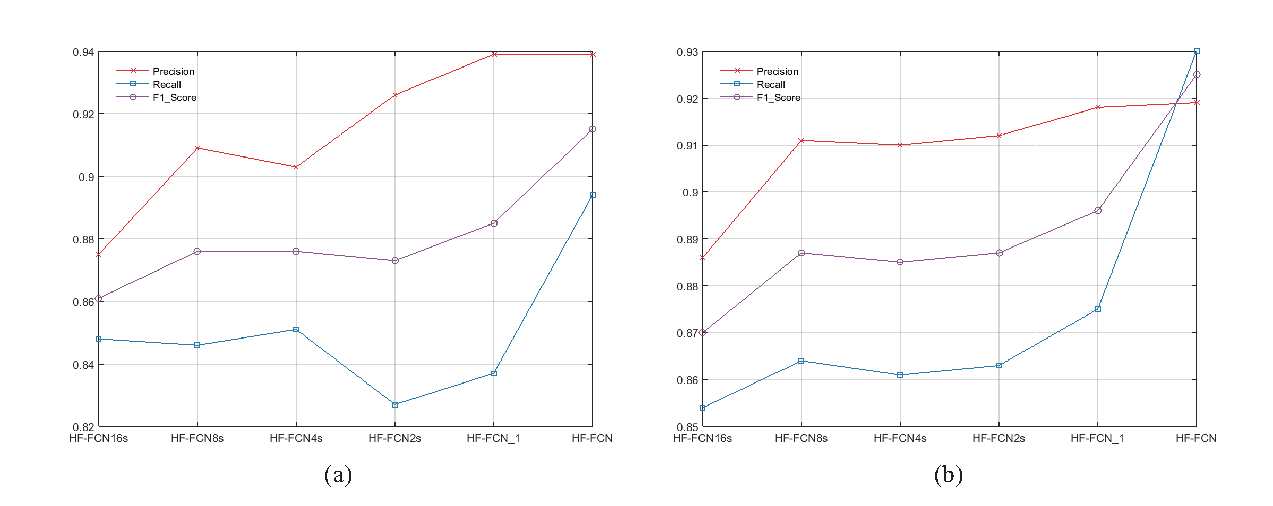
\includegraphics[width=8.7cm]{Figures/vaihingen_variants.eps}
\caption{Results of HF-FCN variants on Vaihingen dataset. (a) (b) shows the precision, recall and F1\_score of validation set and test set of Vaihingen dataset respectively.}
\label{11}
\end{figure}

\begin{figure}
\centering
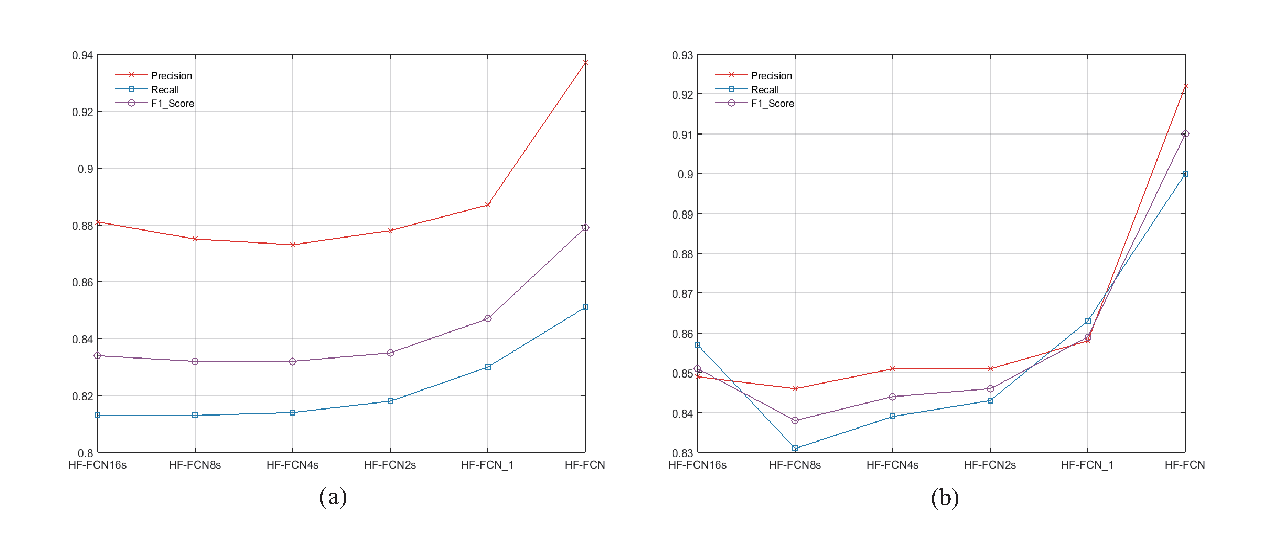
\includegraphics[width=8.7cm]{Figures/Potsdam_variants.eps}
\caption{Results of HF-FCN variants on Potsdam dataset. (a) (b) shows the precision, recall and F1\_score of validation set and test set of Potsdam dataset respectively.}
\label{12}
\end{figure}

\begin{figure}
\centering
\includegraphics[width=8.7cm]{Figures/Vaihingen3_4_5in.eps}
\caption{Prediction results on Vaihingen dataset. (a) (b) (c) shows results of the 3-channel input, 4-channel input and 5-channel input of Vaihingen dataset respectively. Here, TP are shown in green, FP are shown in blue and FN are in red.}
\label{13}
\end{figure}

\begin{figure}
\centering
\includegraphics[width=8.7cm]{Figures/Vaihingen_compared_results.eps}
\caption{Results of different methods. (a) is input image, (b)(d)(g) are results of \cite{IEEEexample:audebert2017deep}, (c) is result of \cite{IEEEexample:marmanis2016semantic}, (f) is result of \cite{IEEEexample:unknown}, (g) is our result.}
\label{14}
\end{figure}

\begin{figure}
\centering
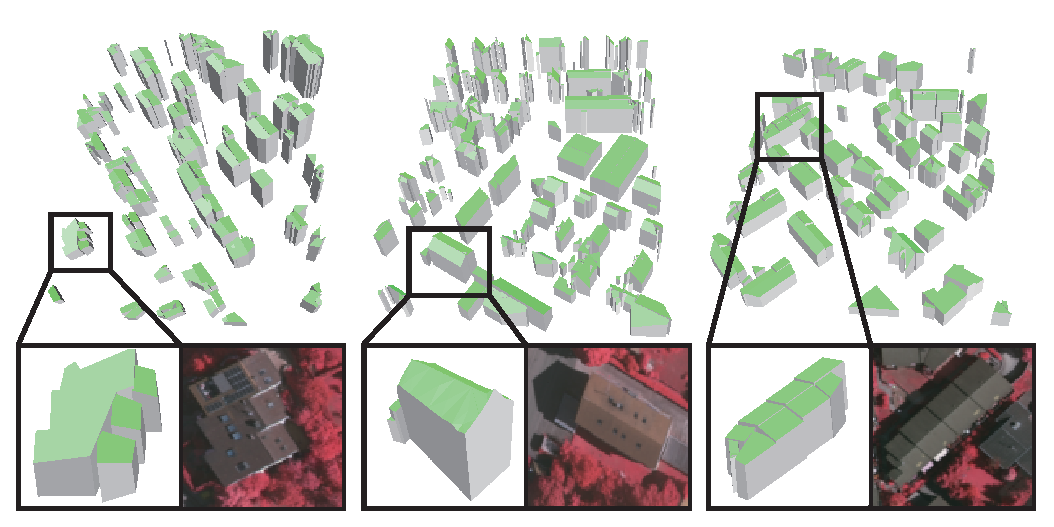
\includegraphics[width=8.7cm]{Figures/Vaihigen_3Dmodelling.eps}
\caption{The 3D modelling of Veihingen dataset. The single building model and its corresponding optical patch were shown together.}
\label{15}
\end{figure}



\subsection{Potsdam dataset}
 The same experiments are implemented on Potsdam dataset. First, We utilize DSM and IR information as extra inputs based on the RGB input. The specific quantitative evaluation and intuitive visual prediction results are shown in Table\Rmnum{7} and Figure 16. In the validation process, the 4-channel input gets better overall performance. Meanwhile, the 5-channel input seems perform better in the course of testing. From the visual results, the 5-channel input network gets lower error detection rate which is shown on the image with small blue areas. And from the 5-channel input to 3-channel input, the F1 score increases from 0.907 to 0.915 on the validation set and increases 0.047 on the test set \par
 \setlength{\parindent}{2ex} As done on Vaihingen dataset, contrast experiments of HF-FCN variants are implemented. The performance curve of HF-FCN variants are shown in Figure 12. We compare HF-FCN with other methods applied to the Potsdam dataset. Some qualitative results are shown in Figure 17. HF-FCN got more remarkable segmentation results while edges and details segmentation of other methods do not perform so good. The same way of 3D city modelling is applied to the Potsdam dataset. Some models of scenes are shown in Figure 18.

\begin{table*}[htbp]
    \caption {Performance comparison of the results of different inputs on Potsdam data set}
    \begin{center}
    \begin{tabular}{p{1.1cm}<{\centering}|p{1.1cm}<{\centering}|p{1.1cm}<{\centering}|p{1.1cm}<{\centering}|p{1.1cm}<{\centering}|p{1.1cm}<{\centering}|p{1.1cm}<{\centering}|p{1.1cm}<{\centering}|p{1.1cm}<{\centering}|p{1.1cm}<{\centering}|p{1.1cm}<{\centering}}
     \hline
    &\multirow{2}{*}{Img}&\multicolumn{3}{c}{3\_in:RGB} &\multicolumn{3}{|c|}{4\_in:RGB,IR}&\multicolumn{3}{c}{5\_in:RGB,IR,nDSM}\\
     \cline{3-11}
    && Pre &Rec & F1 &Pre &Rec &F1&Pre &Rec &F1\\
    \hline\hline
    \multirow{4}{*}{Val}&2\_11&0.917&0.950&0.933&0.917&0.978&0.946&0.934&0.976&0.954\\
    &4\_10&0.937&0.945&0.941&0.926&0.943&0.936&0.947&0.946&0.946\\
    &5\_11&0.930&0.972&0.950&0.959&0.975&0.966&0.956&0.977&0.967\\
    &7\_10&0.964&0.536&0.689&0.950&0.590&0.728&0.939&0.554&0.697\\
    \cline{2-11}
    &{Average}&0.937&0.851&0.879&0.937&$\bm{0.872}$&$\bm{0.894}$&$\bm{0.944}$&0.864&0.891\\
    \hline\hline
    \multirow{3}{*}{Test}&2\_12&0.897&0.868&0.882&0.920&0.959&0.939&0.944&0.965&0.955\\
    &6\_7&0.894&0.902&0.898&0.915&0.909&0.912&0.901&0.918&0.909\\
    &7\_8&0.975&0.929&0.951&0.977&0.950&0.957&0.976&0.946&0.960\\
    \cline{2-11}
    &{Average}&0.922&0.900&0.910&0.937&0.935&0.936&$\bm{0.940}$&$\bm{0.943}$&$\bm{0.941}$\\
    \hline\hline
   \end{tabular}
   \end{center}
   \end{table*}

\begin{figure}
\centering
\includegraphics[width=8.7cm]{Figures/Potsdam3_4_5in.eps}
\caption{Prediction results on potsdam dataset. (a) (b) (c) shows results of the 3-channel input, 4-channel input and 5-channel input of Vaihingen dataset respectively. Here, TP are shown in green, FP are shown in blue and FN are in red.}
\label{16}
\end{figure}

\begin{figure}
\centering
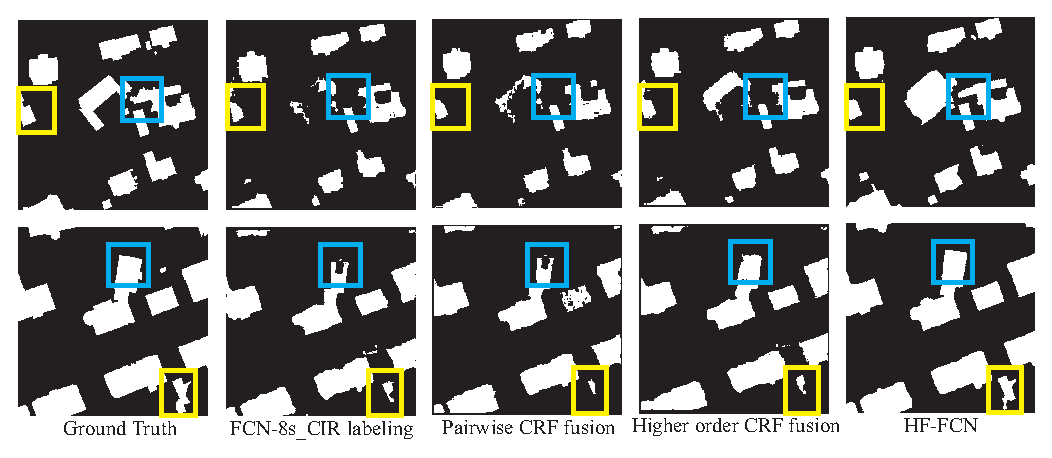
\includegraphics[width=8.7cm]{Figures/Potsdam_compared_results.eps}
\caption{Results of different methods. The second column is the results of using only the FCN with CIR. Pairwise CRF fusion shows the result of fusing FCN-8s\_CIR with LiDAR data in a pairwise CRF. Higher-order CRF are used to generate the results shown in third column. Our results are shown in last colunm.}
\label{17}
\end{figure}

\begin{figure}
\centering
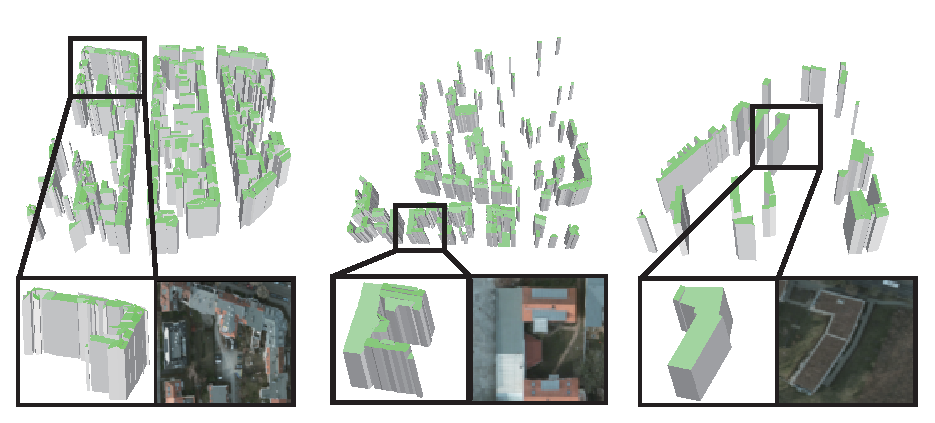
\includegraphics[width=8.7cm]{Figures/potsdam_models.eps}
\caption{The 3D modelling of Potsdam dataset. The single building model and its corresponding optical patch were shown together.}
\label{18}
\end{figure}
